% Chapter3.tex
\chapter{WebDoc - Web Application Documentor}\label{ch:CP}

\begin{figure}[h]
    \centering
    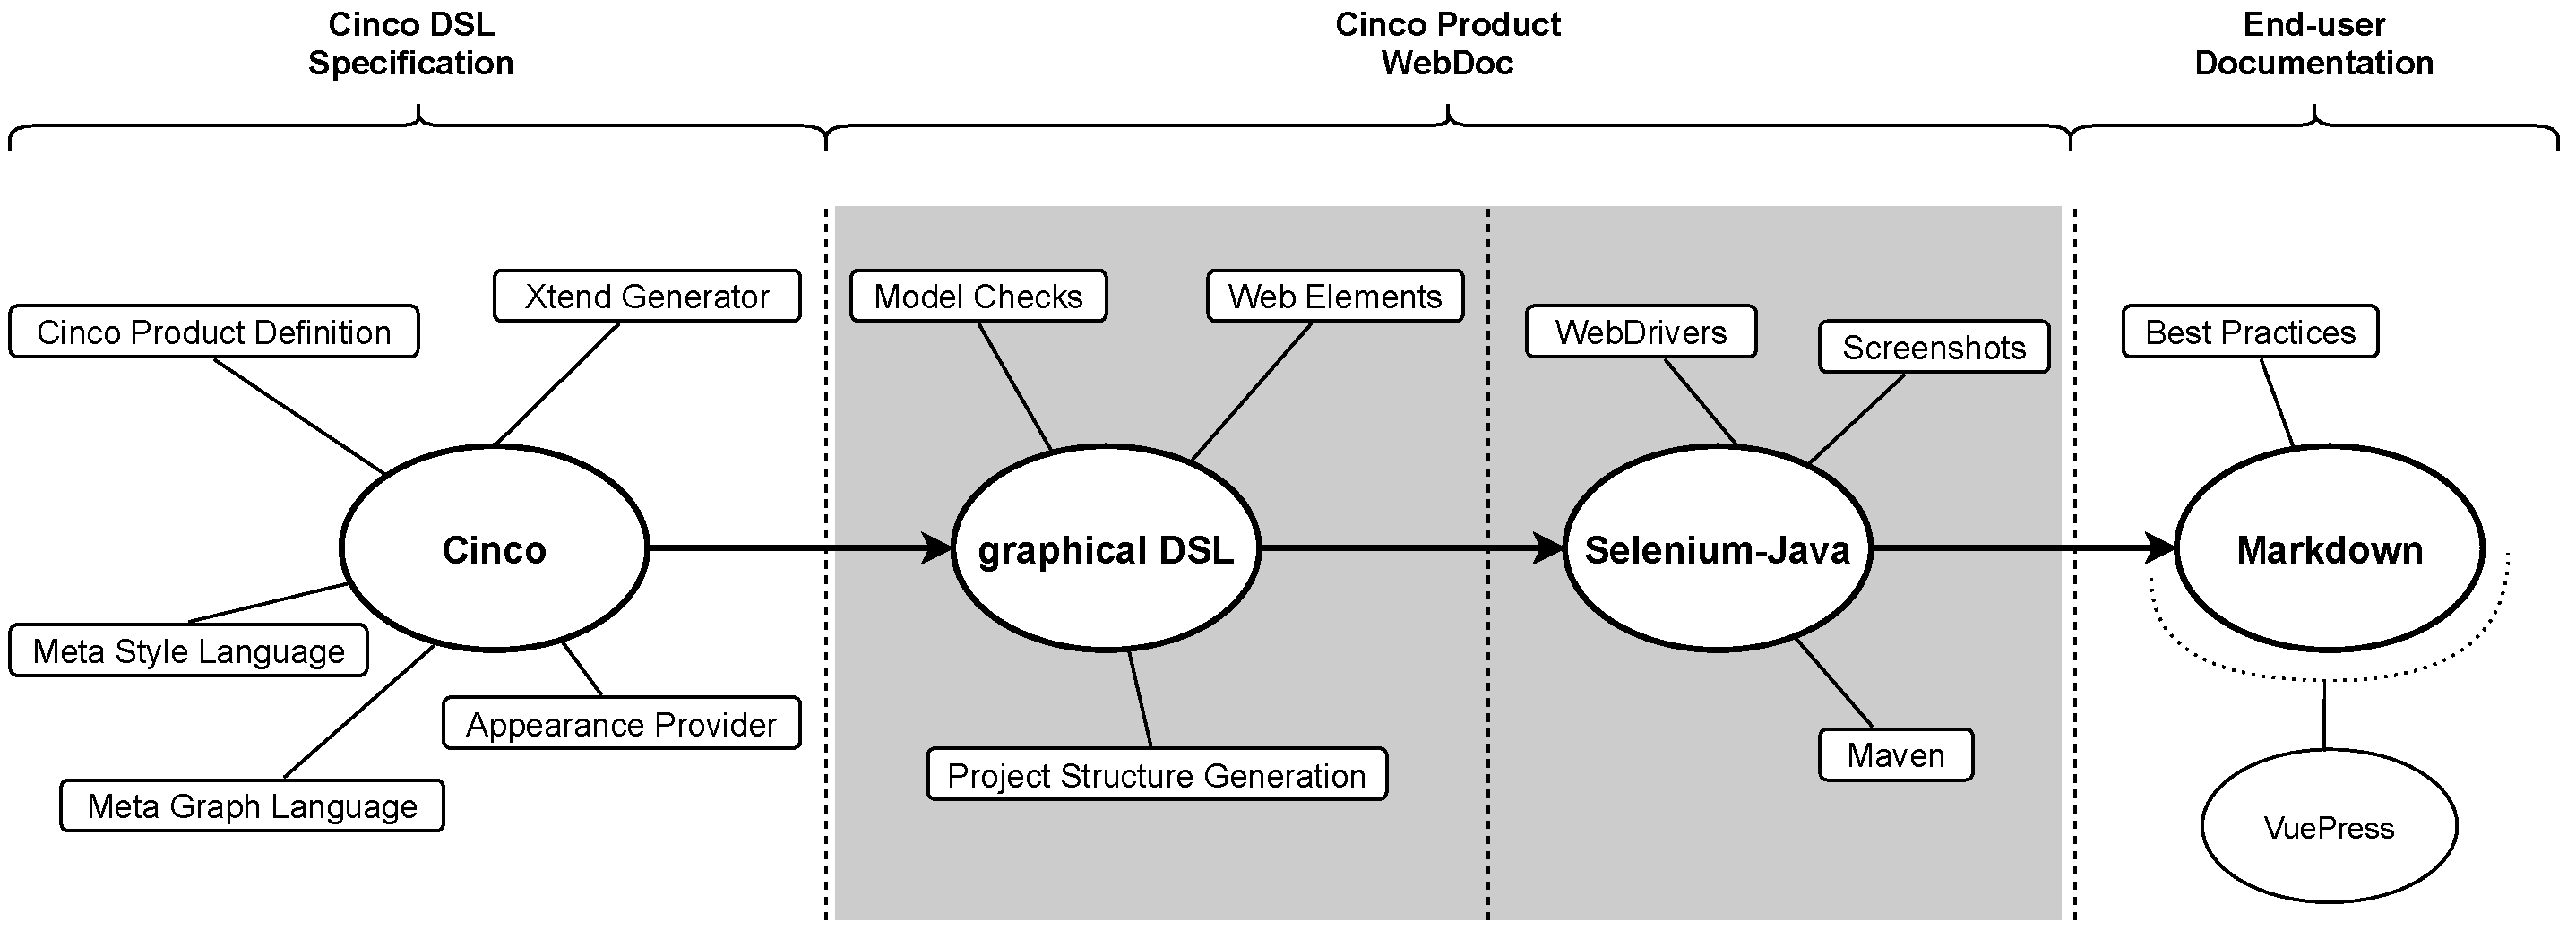
\includegraphics[width=\textwidth]{WebDocDevelopment-gDSL.pdf}
    \label{fig:webDoc}
\end{figure}

Having described the \textsc{Cinco} DSL specification of the graphical modeling tool, we come now to the description of the model editor instantiated from it. First, we give a succinct explanation of our graphical DSL, then illustrate the fundamental building blocks of our documentation model and by presenting at the same time our \textsc{Cinco} product: WebDoc. Later on, we demonstrate the use of these graphical elements to model a specific user workflow on the website we want to document. At the end, we show how using the editor built-in generator, we generate the target application that generate the Markdown files to be shown in the Web browser.

\section{Graphical DSL}\label{sec:gDSL}

Our graphical DSL mainly comprises node elements, which have been applied different appearances to, in order to resemble to some extent the corresponding Web elements they represent, as well as connector elements to connect the nodes to sequence graphs. The purpose behind this approximated replication is not to recreate all possible Web elements, but to give the developer a sense of control over the interactable UI elements. With those elements at hand, the designer can simply model a user action by arranging node elements following the navigation path of the Web application. This graphical language is in such way domain specific, that it is tailored for modeling Web applications inside a Web browser; modeling a documentation for a desktop application for example would not be possible.

\section{Graph Editor}\label{sec:graphEditor}

The WebDoc editor is mainly composed of the canvas in the middle of the working environment (1), where the developer can drag and drop model elements from the palette located on the right-hand side (2). Herein, elements are grouped in categories. On the left-hand side we have the project explorer showing the current project structure (3). The main model files have the extensions .doc and .feat, where the latter is the entry point of the documentation application.

\begin{figure}[h]
    \centering
    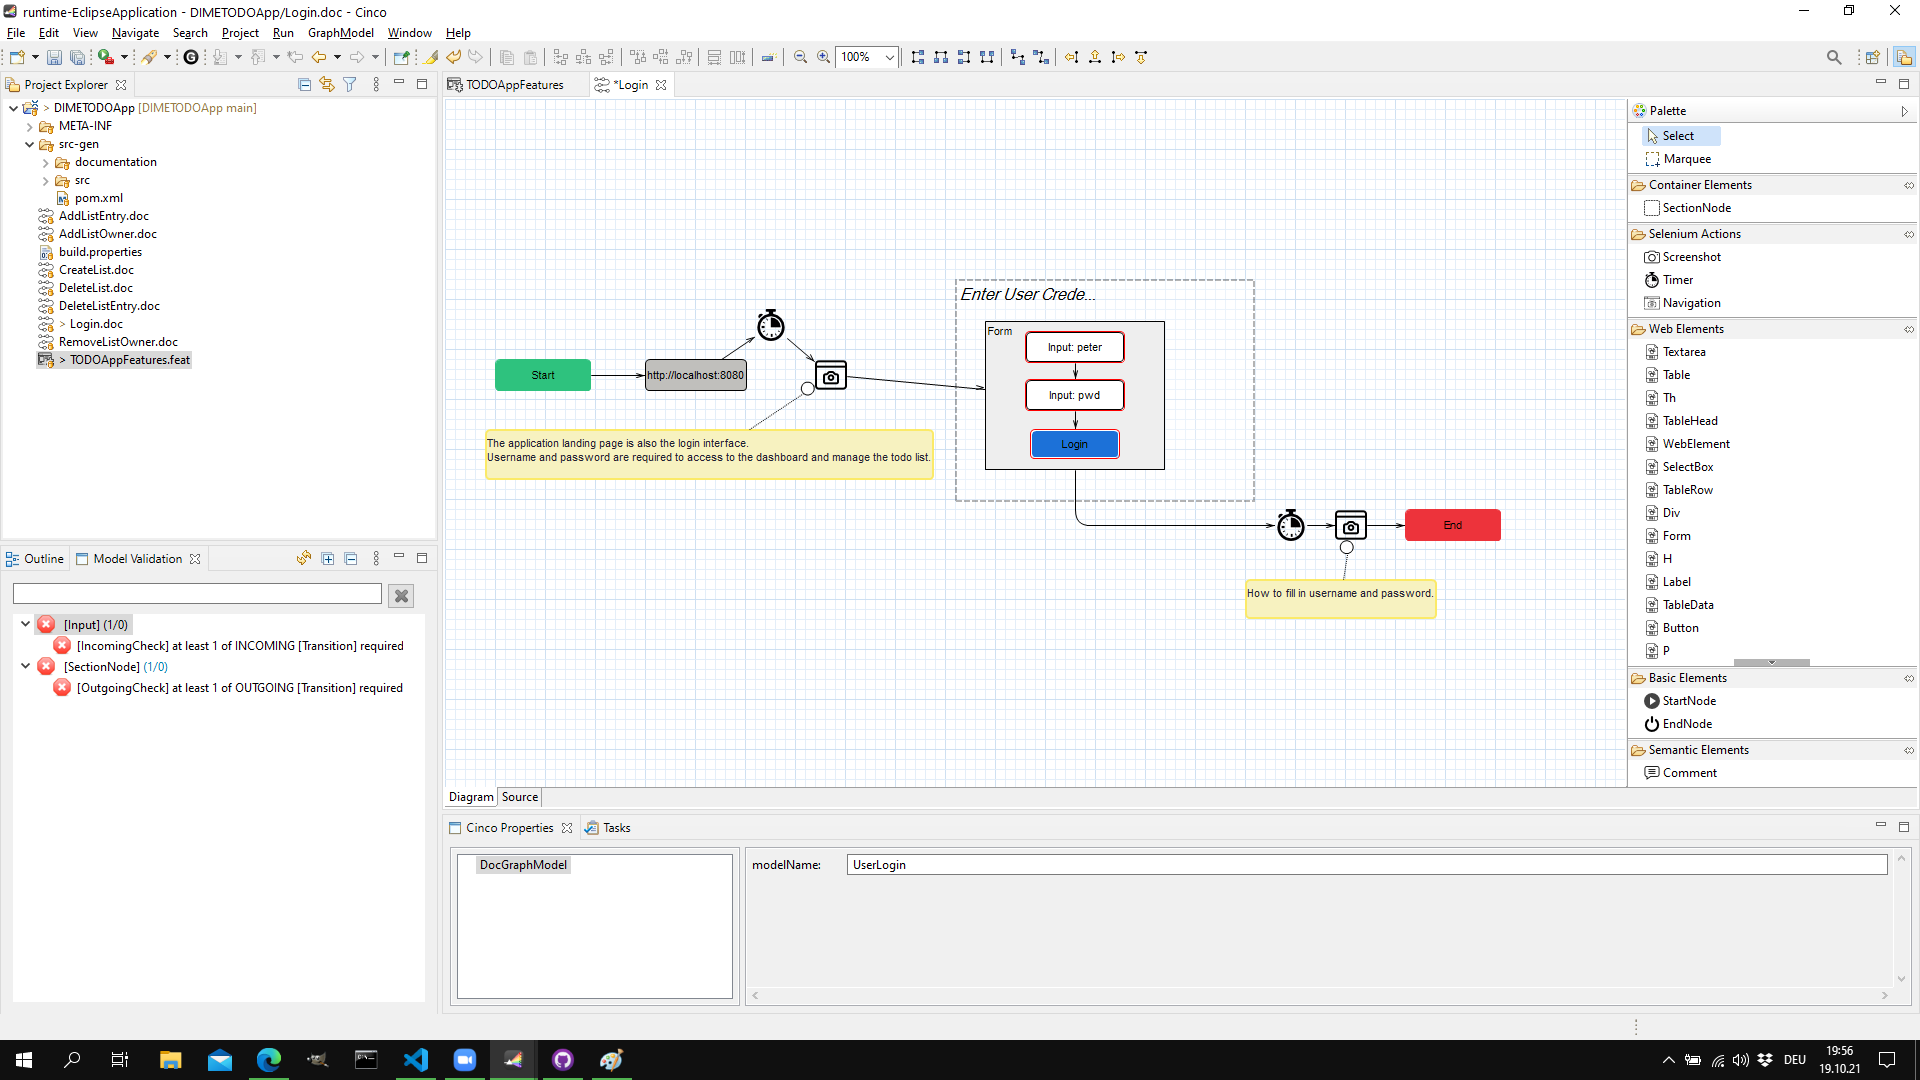
\includegraphics[width=\textwidth]{DocGraphModelChecks.png}
    \caption{\textsc{Cinco} Product Application - Graph model editor}\label{fig:graphDSL}
\end{figure}

All diagrams that are open in the editor are checked in the background for compliance with the requirements described on the metalevel and shown in the Model Checking view right beneath the project explorer (4). There's also the \textsc{Cinco} property view (5) that displays the attributes and values of any selected element in the editor. This is where the developer can modify those values if the attribute field allows it.

\section{WebDoc's Model Elements}\label{sec:WebDocModelElem}

On a Web page rendered in the Web browser, there is a small amount of HTML elements the user can interact with. Most of them resides within the HTML forms, tools that are used for collecting data from the user, or allowing them to control a user interface~\cite{mozillaMDN}. Input fields (of all types: text, password, textarea, checkbox, etc) and buttons are the prominent ones. Those are the Web elements that primarily constitute the palette of our model elements. In the previous chapter, we defined two different \glsplural*{mgl}: one for modeling the Web application features and the other one for modeling the user actions that make up those features.

\subsection{FeatureGraphModel}\label{sec:FeaGrahptModElem}

The FeatureGraphModel is the application starting point specified by the \lstinline{feature.mgl}. Here, the developer groups all the features that needs to be documented in feature containers. Figure~\ref{fig:featGraph} depicts a portion of the features modeled for our task management application: the ability to login, to create a new list, add a task to that list or remove it and lastly delete the whole list. Moreover, our application offers the possibility to also add a new list owner, which already exist in the system as regular user. On the top left-hand corner you can see an property container holding the WebDriver property, whose value is set to \lstinline[language=MGL]{FIREFOX}. It is one of the additional model elements that help the developer define configuration that otherwise could not be modeled, but still essential for the execution of the application. This property value will be assigned to the Selenium WebDriver variable in the Java class. Remember that the executable file for the chosen WebDriver muss already exist somewhere in file system and the path to it has to been specified here in the property view.

\begin{figure}[H]
    \centering
    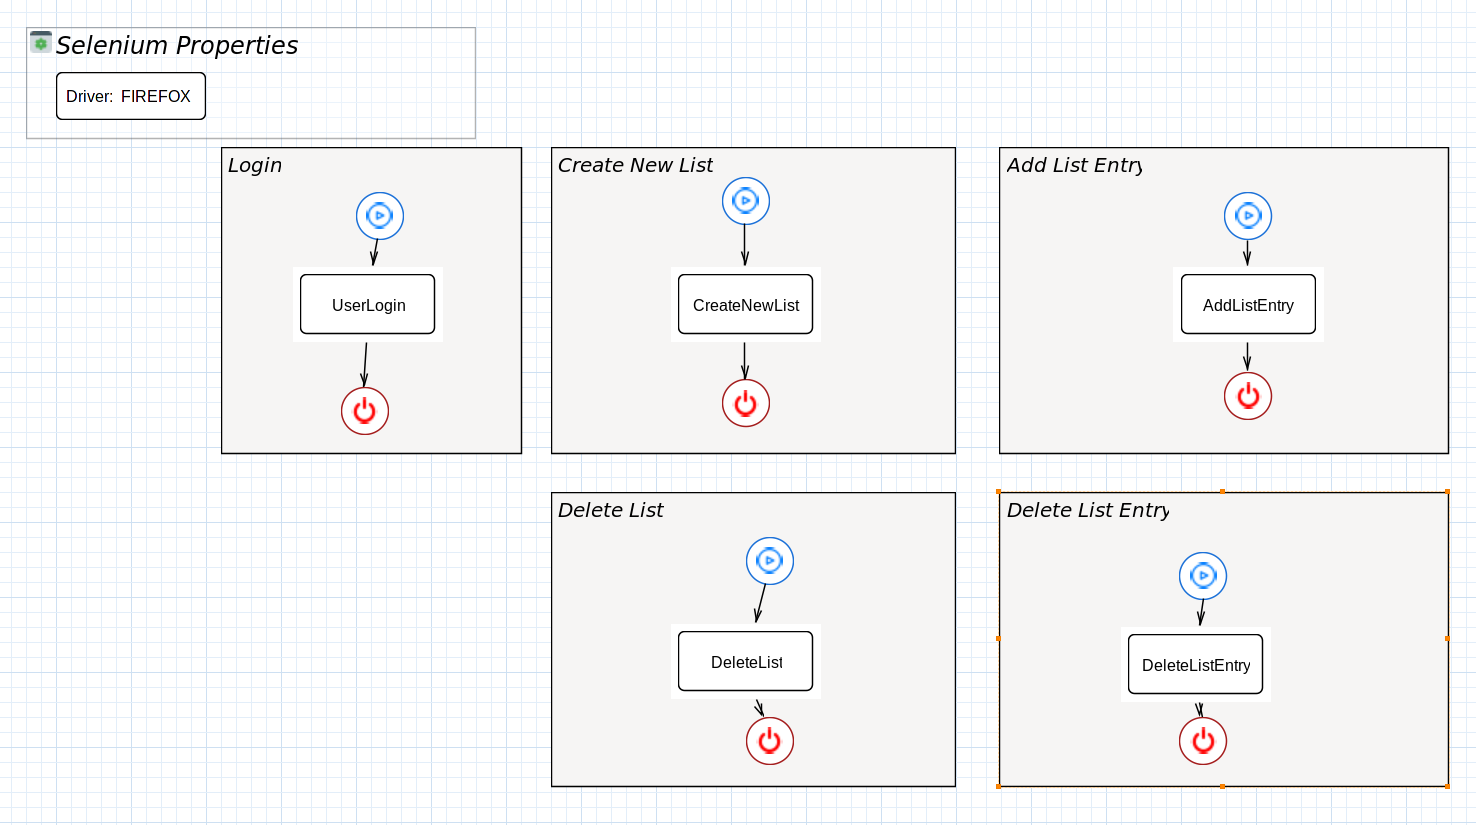
\includegraphics{FeatureGraphModel2.png}
    \caption{\textsc{Cinco} product - Feature Graph Model with Feature Containers}
    \label{fig:featGraph}
\end{figure}

Even though the features are presented in logical workflow order, they still are independent from one another and will be generated independently as well. However, as mentioned in the previous chapter, this separation does not exclude reusability, since it is possible to integrate a whole DocGraphModel inside another one. Considering, for instance, the CreateNewList feature, it requires the user to be logged in to be able to create a new tasks list. So the documentation developer does not have to repeat the login sequence inside the this one and can simply drag and drop the UserLogin.doc file inside the diagram of the new model graph, connect it within the sequence as if it were a regular graph node (see figure~\ref{fig:reusability}). Double-clicking on the imported subgraph leads directly to the original graph model. This double-click action has been implemented by applying the \lstinline[language=MGL]{@doubleClickAction} annotation the corresponding node specification and by providing a custom action class that holds the implementation logic.

\begin{figure}[h]
    \centering
    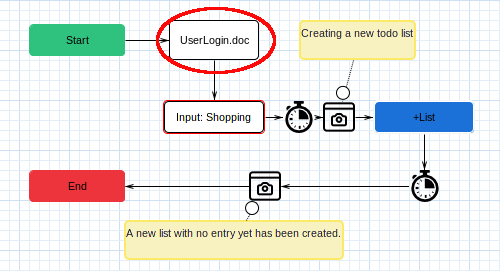
\includegraphics[width=\textwidth]{Reusability.png}
    \caption{\textsc{Cinco} product - Reusing Login graph model in the CreateNewList graph model}
    \label{fig:reusability}
\end{figure}

The feature graph model contains also semantic elements, which are integrated in the existing featureContainer for simplicity's sake. Clicking on such a featureContainer opens up simultaneously the Cinco property view with a multiline input field \lstinline{description}. This is where the documentation designer can enter some descriptive text to give meaning to the diagram elements and at the same time provide text content for the Markdown documentation files. Those information will be collected during the code generation process.

\subsection{DocGraphModel}\label{sec:DocGrahpModElem}

The model in Figure~\ref{fig:loginSeq} illustrates the sequence a user would eventually undergo to log into our example Web application, with the Web elements that will be interacted with. Connected together into a logical sequence, they form the user login sequence for our Web application. 

The sequence begins with the start node, which is the starting point of every user sequence, then comes the navigation node, used to navigate from one Web page to another. Next, the timer node waits explicitly for an amount of second  determined by the designer in the property view and for a certain condition to become true before continuing. Those ExpectedConditions are i.e. \lstinline{presenceOfElementLocated}, \lstinline{elementToBeClickable}, just to name a few. If we take for example the condition \lstinline{presenceOfElementLocated}, the timer holds the WebDriver execution for 3 seconds, checking every 500 milliseconds if the targeted Web element appears on the page. Right after the timer comes the Screenshot node, that captures the current application state, displaying the application landing page, also the login pane. In the property view, one can give a specific file name to each image that has to be saved. The comment node allows the documentation creator to add descriptive text about the picture, that will be later added to the Markdown file as image caption. Next comes a section describing the action of typing in and validating the user credentials. As you can hopefully see, all input node, as well as the button node have a red border that simulates the element state of being highlighted. This visual help show the model designer which elements will be marked on the next screenshot, after which the login sequence ends.
\begin{figure}[h]
    \centering
    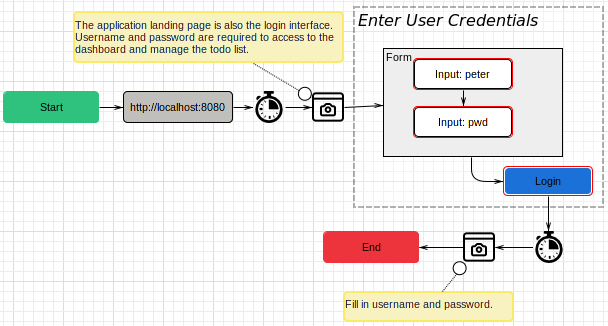
\includegraphics{WebDoc-graphModel.png}
    \caption{Example of a user workflow: here the login sequence}
    \label{fig:loginSeq}
\end{figure}

The purpose of the Web element nodes is to allow the concrete \gls*{html} elements in the browser to be addressed. This implies that appropriate actions can be applied to such a representation of an \gls*{html} element. Considering for instance the input field in the picture below, the action of typing in a text is made possible by providing a property variable \lstinline{content}, whose value is then display inside the node element (here i.e. ''peter'' and ''pwd''). The same holds true for button elements, which can be applied the click action or for selectboxes, which can be dropped down to reveal the options they contain, etc. In addition to that, all Web element can be highlighted either by setting the \lstinline{highlighted} property to true or by letting the Highlight node under the \textit{Selenium Actions} category take care of it. 

\section{Graph Model Checks}\label{sec:modCheck}

Modeling valid graph diagrams is crucial for the correctness of the generated application code. Especially the Selenium-Java application code has to replicate correctly the user sequence in order capture the correct application state as the user would do. This is particularly daunting if the navigation graph of the underlying Web application is huge.

This means that we have to ensure that there is a distinct for every single using action or that there is no cycle within such path. This strongly reminds of some graph theory problems: checking is a path from start to end node exists and whether or not a given graph is cycle free. The \textsc{Cinco} framework offers a meta plugin ready-to-go for this task, the MCaM Meta Plugin~\cite{gitlabcinco}. The plugin has to be activated by specifying the \lstinline{@mcam("...")} annotation with the corresponding parameter in parentheses.

check also that screenshot files do not have the identical file name
\section{Generation Process}\label{sec:GenProcess}

\begin{figure}[h]
    \centering
    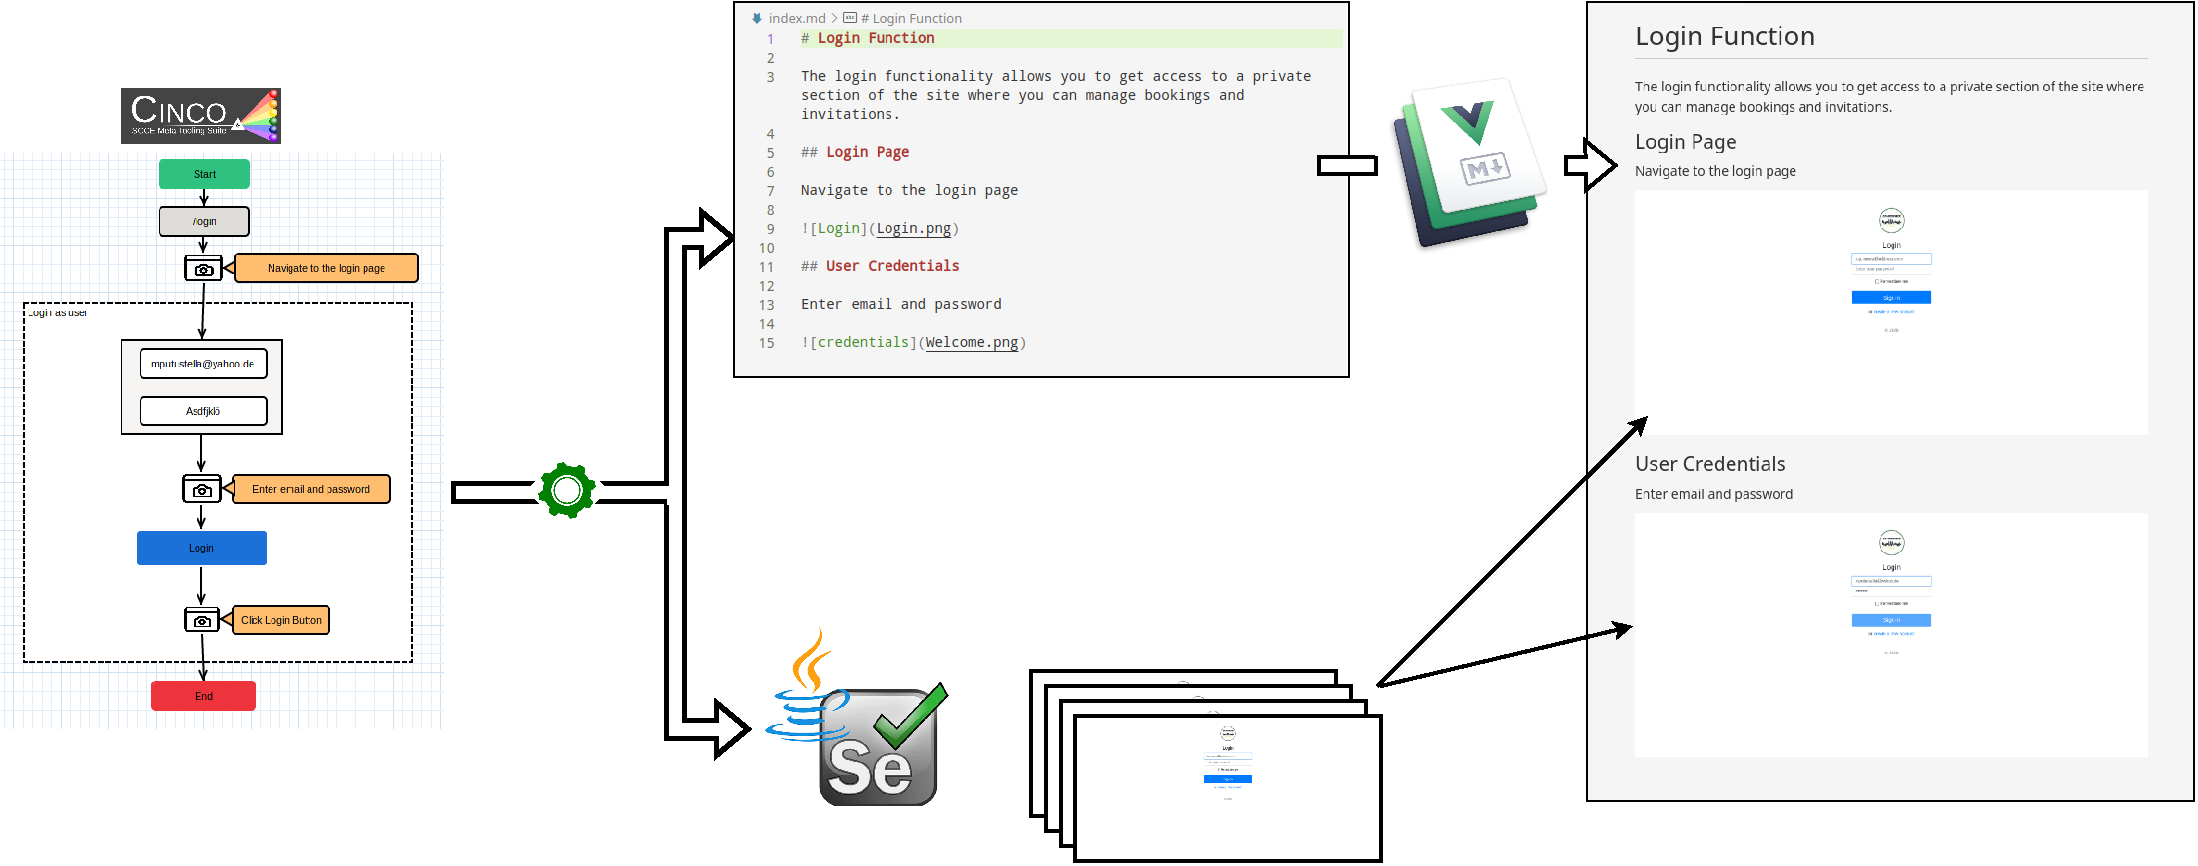
\includegraphics[width=\textwidth]{WebDoc-workflow.pdf}
    \caption{End user Documentation generation process}
    \label{fig:WebDocWorkflow}
\end{figure}

As mentioned before, the prominent feature of \textsc{Cinco} is the generate button. This allows the developer, after the modeled has been laid out without errors, to generate the a fully realized Selenium-Java application, which is going to execute the user sequence model just created. Figure~\ref{fig:genButton} shows where the generate button is located.

\begin{figure}[H]
    \centering
    
\includegraphics[width=\textwidth]{GenerateButtonHighlighted.png}
    \caption{\textsc{Cinco} product - generator button}
    \label{fig:genButton}
\end{figure}
